\documentclass{beamer}

\usepackage{ucs}
\usepackage[utf8x]{inputenc}
\usepackage[T1]{fontenc}
\usepackage[english]{babel}

\usepackage{multirow}%	multirow
\usepackage[retainorgcmds]{IEEEtrantools}%	IEEEeqnarray
\usepackage{mathabx}%	convolution symbol
\usepackage{relsize}%	relative font sizes
%\usepackage{enumitem}

%	presentation info
\title{Profiling + CUDA}
\subtitle{A finite volume case study from an industrial application\\\smaller Shared Memory with OpenMP}

\author{Miguel Palhas}

\institute[pg19808]{
	University of Minho \\
	Department of Informatics
}

\date{Braga, January 2012}


%	beamer options
\usetheme{CambridgeUS}

\begin{document}%	begin presentation

\maketitle%	title slide

\begin{frame}
	\frametitle{Index}
	%\begin{multicol}{2}
	\tableofcontents
	%\end{multicol}
\end{frame}

\section{Data Structures}
\begin{frame}
	\begin{center}
		\Huge{Data Structures}
	\end{center}
\end{frame}

\begin{frame}
	\frametitle{Data structures}

	\begin{itemize}
		\item Current FVLib implementation is not suitable for CUDA.
		\item[]
		\item All mesh data is based on dereferencing strategies (lots of pointers!).
		\item[]
		\item All relevant data structures need to be re-written:
		\begin{itemize}
			\item Avoid pointers,
			\item Convert to Struct-of-arrays,
		\end{itemize}
	\end{itemize}
\end{frame}

\section{Implementation}
\begin{frame}
	\begin{center}
		\Huge{Implementation}
	\end{center}
\end{frame}

\begin{frame}
	\frametitle{Implementation}

	\begin{itemize}
		\item[] No improvement when using GPU only for \texttt{compute\_flux}.
		\begin{itemize}
			\item Requires a memcpy every iteration.
			% not all data requires copy, but enough to create overhead.
			% I don't have the actual number, but i tested after first implementing compute_flux and believe me, it was slow.
		\end{itemize}
		\item[]
		\item[] Full GPU implementation of the main loop required. But not with a single kernel:
		\begin{itemize}
			\item After each phase, global synchronization is required; % syncthreads only syncs within a block
			\item Optimal number of blocks/threads/registers differs for each operation;
		\end{itemize}
		\item[]
		\item[] Kernels required: \texttt{compute\_flux}, \texttt{reduction}, \texttt{update}.
	\end{itemize}
\end{frame}

\begin{frame}
	\frametitle{Implementation}

	\begin{itemize}
		\item \texttt{compute\_flux: } Implementation based on original version. \\
			Each CUDA Thread computes flux for a single edge, and it's velocity.
		\item[]
		\item \texttt{reduction: } Reduces all velocities to find max absolute value. \\
			Based on most optimized version from NVidia samples.
	\end{itemize}
\end{frame}

\begin{frame}
	\frametitle{Implementation - Update}

	\begin{itemize}
		\item[] Original version iterates through all the edges, updating values for left and right cell.
		\item[] When parallelizing, multiple threads might be updating the same cell, creating data races.
		\item[]
		\item[] Implemented kernel iterates through the cells, eliminating the problem.
	\end{itemize}
\end{frame}

\section{Profiling}

\begin{frame}
	\begin{center}
		\Huge{Profiling}
	\end{center}
\end{frame}

\begin{frame}
	\frametitle{Profiling - Methodology}

	\begin{itemize}
		\item PBS job to run all tests
		\item Full node requested
		\item Kernel times measured with Cuda Events, and profiling disabled
		\begin{itemize}
			\item[] All kernels become synchronous when profiler is enabled
		\end{itemize}
		\item All values are the counters's average for each iteration
		\item[]
	\end{itemize}

\end{frame}

\begin{frame}
	\frametitle{Kernel Execution Time}

	\begin{figure}[!htp]
		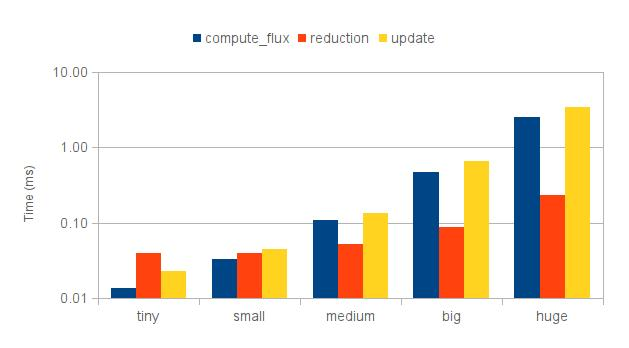
\includegraphics[width=0.8\textwidth]{images/cuda_kernels}
		\label{fig:kernels}
		\caption[Kernel execution time]{Execution time for each kernel}
	\end{figure}
\end{frame}

\begin{frame}
	\frametitle{Compute Flux Comparison}

	\begin{figure}[!htp]
		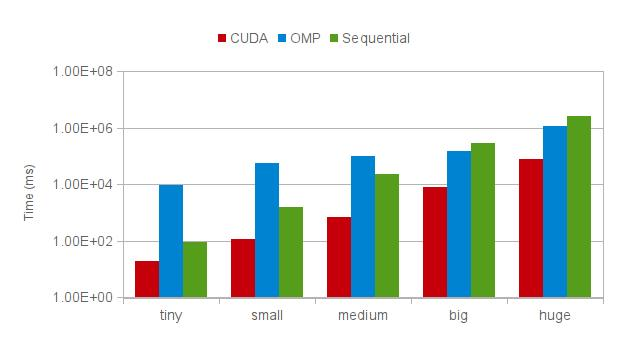
\includegraphics[width=0.8\textwidth]{images/cuda_omp_compute_flux}
		\label{fig:compute_flux}
		\caption{CUDA vs OMP - \texttt{compute\_flux}}
	\end{figure}
\end{frame}

\begin{frame}
	\frametitle{Program Execution Time}

	\begin{figure}[!htp]
		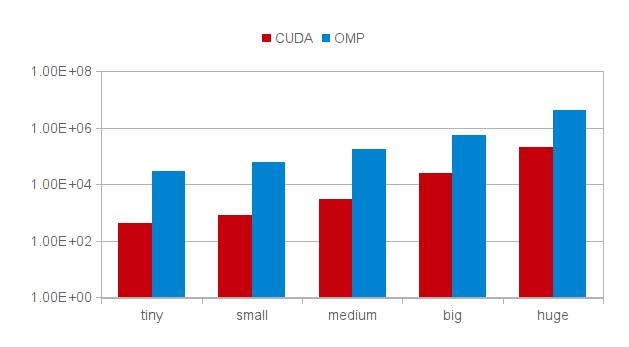
\includegraphics[width=0.8\textwidth]{images/cuda_omp_global}
		\label{fig:full_time}
		\caption{CUDA vs OMP - Program execution time}
	\end{figure}
\end{frame}

\section{Conclusions}
\begin{frame}
	\begin{center}
		\Huge{Conclusions}
	\end{center}
\end{frame}

\begin{frame}
	\frametitle{Conclusions}

	\begin{itemize}
		\item CUDA implementation is much faster, but also more optimized;
		\begin{itemize}
			\item[] Bigger inputs are required to better understand scalability;
		\end{itemize}
		\item[]
		\item Both versions still have room for improvement
		\begin{itemize}
			\item[] Data structures optimization is essential!
		\end{itemize}
		\item[]
		\item Data organization has a significant impact on performance;
		\item[]
		\item CUDA Profiler is not suited for CPU vs GPU comparison, but for measuring impact of optimizations between CUDA implementations.
	\end{itemize}
\end{frame}

\begin{frame}
	\frametitle{Future Work}

	\begin{itemize}
		\item Review of the data structures
		\item Review of FVLib classes
		\item Analyse scalability with greater input sizes (hard to generate)
		\item Usage of CUDA Streams
		\item Analyse usage of shared memory
		\item Optimize performance with animation output (biggest bottleneck when enabled)
	\end{itemize}
\end{frame}

%\section{Algorithm}
%\subsection{Definition}
%\begin{frame}%	begin slide
%	\frametitle{Convolution}
%	%	from Wolfram: http://mathworld.wolfram.com/Convolution.html
%	\begin{quote}
%		\cite{wolfram} A \textbf{convolution} is an integral that expresses the amount of overlap of one function  as it is shifted over another function . (\ldots) The convolution is sometimes also known by its German name, faltung ("folding").
%	\end{quote}
%	\begin{IEEEeqnarray}{C}
%		\left [ f\convolution g \right ] = \int^{t}_{0}{f(\tau)\;g(t-\tau)\;d\tau}
%	\end{IEEEeqnarray}
%	Specific cases:
%	\begin{itemize}
%		\item{2-D Convolution (Images)}
%	\end{itemize}
%\end{frame}%	end slide
%
%\subsection{Discrete}
%\begin{frame}
%	\frametitle{Discrete Convolution}
%	\begin{figure}
%		\includegraphics{images/convolution.png}
%	\end{figure}
%	\begin{IEEEeqnarray}{C}
%		\forall r_{ij}\in R,\enspace r_{ij} = \sum_{y}\sum_{x} k_{yx}\times m_{zw}
%	\end{IEEEeqnarray}
%	\begin{description}
%		\item[where]{$z = i + y - a$}
%		\item[and]{$w = j + x - b$}
%		\item[and]{$k_{ab}$ is the center of K.}
%	\end{description}
%\end{frame}
%
%\section{Hardware profile}
%\subsection{MacBook Pro}
%\begin{frame}
%	\frametitle{Hardware profile}
%	Apple MacBook Pro 6,2
%	\begin{itemize}
%		\item{Intel i5-540M 2.4 GHz;}
%		\item{One processor;}
%		\item{Two cores;}
%		\item{L1 cache 32 KB + 32 KB, per core;}
%		\item{L2 cache 256 KB, per core;}
%		\item{L3 cache 3 MB, shared;}
%		\item{4GB RAM DDR3 1067 MHz;}
%	\end{itemize}
%\end{frame}
%
%\begin{frame}
%	\frametitle{Roofline}
%	\begin{figure}
%		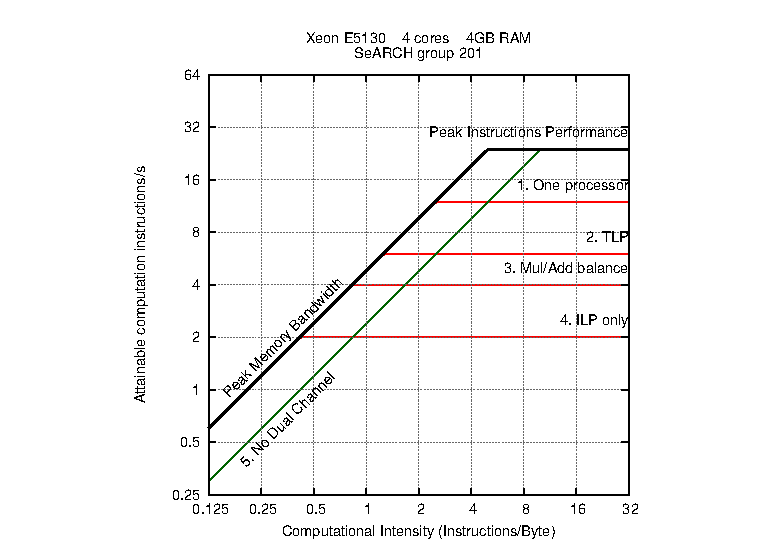
\includegraphics[width=10cm]{plot/roofline.eps}
%	\end{figure}
%\end{frame}
%
%\subsection{SeARCH Node 201-1}
%\begin{frame}
%	\frametitle{Hardware profile}
%	SeARCH Node 201-1:
%	\begin{itemize}
%		\item{Intel Xeon 5130 2.0 GHz;}
%		\item{Two processors;}
%		\item{Four cores;}
%		\item{L1 cache 32KB + 32KB, 8-way associative;}
%		\item{L2 cache 4MB, 16-way associative;}
%		\item{4GB RAM;}
%	\end{itemize}
%\end{frame}
%
%
%\section{Testing}
%\subsection{Cases}
%\begin{frame}
%	\frametitle{Test cases}
%	\begin{table}
%		\begin{tabular}{|ccc|}
%			\hline
%			\textbf{Memory level} & \textbf{Size} & \textbf{Matrix}	\\
%			\hline\hline
%			\multirow{2}{*}{L1} & 2 KB & $16\times 16$	\\
%			& 8 KB & $32\times 32$	\\
%			\hline\hline
%			\multirow{2}{*}{L2} & 512 KB & $256\times 256$	\\
%			& 2 MB & $512\times 512$	\\
%			\hline\hline
%			\multirow{2}{*}{RAM} & 8 MB & $1024\times 1024$	\\
%			& 32 MB & $2048\times 2048$	\\
%%			& 2 GB & $16384\times 16384$	\\
%			\hline
%		\end{tabular}
%	\end{table}
%	To compare the results more easily, the kernel size is fixed to $9\times 9$ (648 B).
%\end{frame}
%
%\subsection{Counters}
%\begin{frame}
%	\frametitle{Hardware Counters}
%	
%	\begin{enumerate}
%		\item{Instructions:
%		\begin{itemize}
%			\item{Total;}
%			\item{Load \& store;}
%			\item{Floating point (total, SP \& DP);}
%			\item{SIMD (total, SP \& DP);}
%		\end{itemize}
%		}
%		\item{Memory:
%		\begin{itemize}
%			\item{L1 data cache (access, hit \& miss);}
%			\item{L2 data cache (access, hit \& miss);}
%		\end{itemize}
%		}
%		\item{Operations:
%		\begin{itemize}
%			\item{Floating point (total, SP \& DP).}
%		\end{itemize}
%		}
%	\end{enumerate}
%	On SeARCH Node 201-1, the counter for L2 data cache hit was replaced with the counters for total L2 hits and for L2 instruction hits.
%\end{frame}
%
%\subsection{Methodology}
%\begin{frame}
%	\frametitle{Methodology}
%	\begin{itemize}
%		\item{Best three runs in a range no larger than 5\%;}
%		\item{One execution per counter on every run;}
%		\item{Every run the total number of cycles is measured;}
%		\item{$T_{\mathrm{run}} = \overline{e}$;}
%	\end{itemize}
%\end{frame}
%
%\begin{frame}
%	\frametitle{Methodology}
%	\begin{center}
%		\textbf{\LARGE !!! Important !!!}
%		
%		Every execution must be a different process
%		
%		\underline{cache warm up}
%	\end{center}
%\end{frame}
%
%\section{Results}
%\subsection{General}
%\begin{frame}
%	\frametitle{Results}
%	\begin{itemize}
%		\item{25\% to 28\% memory accesses per instruction;}
%		\item{95\% to 99\% ADD/MUL balance;}
%		%\item{≈ 0.03 CPI $\Leftrightarrow$ ≈ 30 IPC;}
%		\item{Cache warm up problems on cache levels cases:
%		\begin{itemize}
%			\item[!]{Infinite operational intensity;}
%			\item[!]{Very close access and hit values;}
%		\end{itemize}
%		}
%		\item{On higher levels:
%		\begin{itemize}
%			\item{10 Flops/Byte operational intensity;}
%			\item{75 instructions / Byte of RAM;}
%		\end{itemize}
%		}
%	\end{itemize}
%\end{frame}
%
%\subsection{Instructions per byte of RAM read}
%\begin{frame}
%	\frametitle{\# Instructions / RAM bytes read}% #inst / byte to ram
%	\begin{figure}
%		\includegraphics[width=11cm]{images/instbyteram.png}
%	\end{figure}
%	Cache level cases tended to infinite.
%\end{frame}
%
%\subsection{Miss rates}
%\begin{frame}
%	\frametitle{Miss rates}% %miss / case size
%	\begin{figure}
%		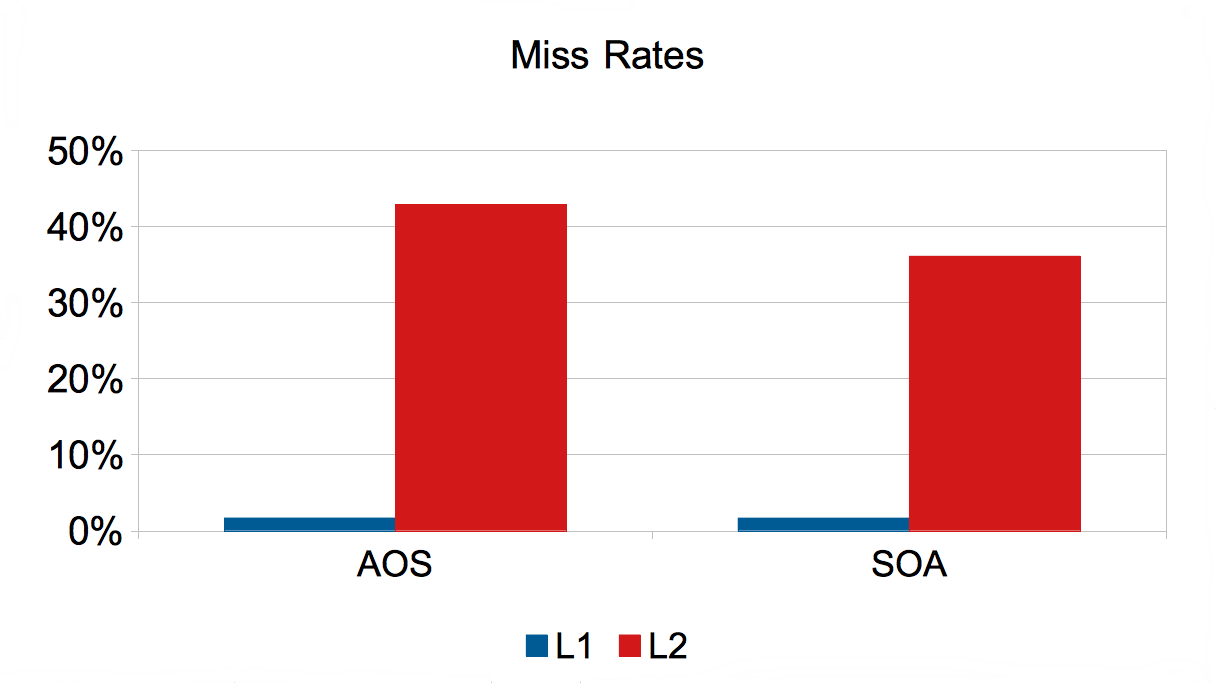
\includegraphics[width=12cm]{images/missrates.png}
%	\end{figure}
%\end{frame}
%
%\section{Conclusion}
%\begin{frame}
%	\frametitle{Conclusion}
%	\begin{itemize}
%		\item{Simplifications have consequences.%	cache warm up
%		\begin{itemize}
%			\item[$\Rightarrow$]{Each execution must be a distinct process.}
%		\end{itemize}
%		}
%		\item{PAPI is not absolute.}
%	\end{itemize}
%\end{frame}
%
%\section{References}
%\begin{frame}
%	\frametitle{References}
%	\begin{thebibliography}{}
%		%	Wolfram
%		\bibitem[Wolfram MathWorld]{wolfram}
%			Weisstein, Eric W.
%			\newblock {\itshape ``Convolution''}
%			\newblock MathWorld -- A Wolfram Web Resource
%			\newblock http://mathworld.wolfram.com/Convolution.html
%	\end{thebibliography}
%\end{frame}
%
\section{Questions}
\begin{frame}
	\titlepage
	\begin{center}
		\Huge\bfseries
		- ? -
	\end{center}
\end{frame}

\end{document}%	end presentation
